\begin{defnbox}\nospacing
  \begin{defn}[Liskov Substitution Principle]\label{defn:}
    If S is a subtype of T, then objects of type T may be replaced with objects of type S \imp{without} altering the correctness of the program
  \end{defn}
\end{defnbox}
\begin{sectionbox}\nospacing
  \begin{wrapfigure}{r}{0.3\linewidth}
		\centering
		\vspace{-10pt}
		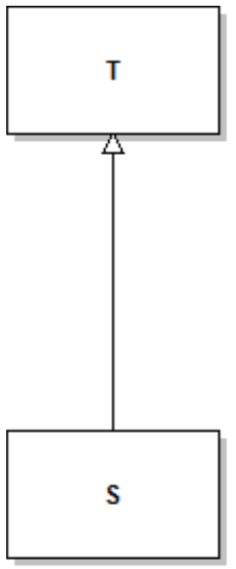
\includegraphics[width=0.55\linewidth]{figures/intro/Lis.png}
  \end{wrapfigure}
  \imp{In other words}:
  \begin{itemizenosep}
      \item Whenever you work with an instance of type T, you should not be
    surprised if you effectively work with an instance of type S
      \item An instance of type S can be used at all places where an instance of type T is expected
  \end{itemizenosep}
  \imp{Consequences}: Overriding methods need to satisfy (at least) the rules specified by the base class
\end{sectionbox}
\begin{defnbox}\nospacing
  \begin{defn}[Variance]\label{defn:Variance}
    Is a term applied to the expected behavior of subtypes in a class hierarchy containing complex types.
  \end{defn}
\end{defnbox}

%%% Local Variables:
%%% mode: latex
%%% TeX-master: "../formulary"
%%% End:
